\chapter{Cronograma de actividades}

El desarrollo del proyecto se organiza mediante un cronograma de actividades
distribuido a lo largo del periodo disponible. La planificación se
estructuró considerando las etapas necesarias para pasar desde la definición del
alcance hasta la defensa final del proyecto, procurando mantener una secuencia
realista entre el diseño, la integración de subsistemas, las pruebas y los
ajustes finales.

El cronograma propuesto contempla inicialmente un periodo de retroalimentación y
ajuste del alcance, con el fin de incorporar las observaciones realizadas por
los profesores y delimitar con mayor claridad las funcionalidades que formarán
parte del prototipo. Durante esta misma etapa se considera la investigación
bibliográfica complementaria y la definición de requerimientos, ya que las
observaciones recibidas pueden implicar la revisión de fuentes técnicas,
criterios de diseño, restricciones del sistema o métricas de validación.
La definición de requerimientos permite traducir dichas observaciones en 
criterios concretos de funcionamiento, integración y validación del prototipo.

Una vez definidos los requerimientos, se plantea el diseño de la arquitectura
general del sistema, incluyendo la relación entre el probador ESD comercial, los
módulos de identificación, la interfaz gráfica, el almacenamiento local y los
elementos de integración electrónica. De forma paralela, se considera la
adquisición de componentes, debido a que la disponibilidad de los módulos puede
influir directamente en el avance de la etapa de implementación.

La fase de implementación se concentra en la integración general de los
subsistemas y en el desarrollo de las funcionalidades principales del prototipo.
Dentro de esta etapa se incluyen la identificación por código de barras, el
reconocimiento facial, la interfaz gráfica y el sistema de almacenamiento y
generación de registros. Estas actividades se planifican de forma parcialmente
traslapada, ya que algunos subsistemas pueden desarrollarse en paralelo siempre
que se encuentren definidos los protocolos de comunicación y la estructura
general de datos.

Finalmente, el cronograma incluye una etapa de pruebas funcionales, validación
del sistema, ajustes finales, documentación y defensa. Esta distribución permite
reservar tiempo para corregir errores detectados durante la integración,
verificar el cumplimiento de los criterios de aceptación y consolidar la
evidencia técnica necesaria para el informe final del proyecto.

\begin{figure}[H]
    \centering
    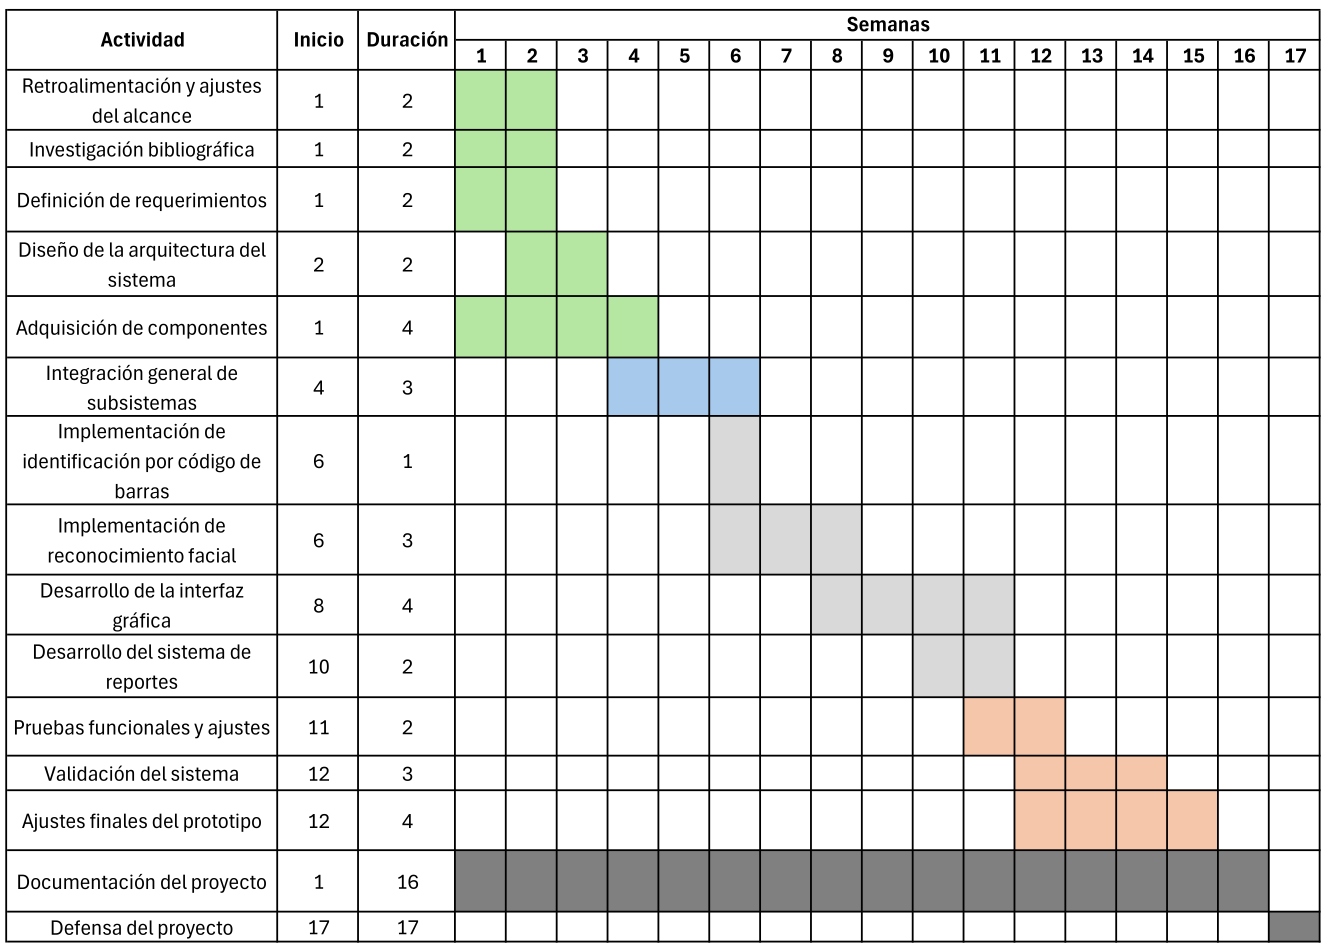
\includegraphics[width=\textwidth]{pics/SP_21.png}
    \caption{Cronograma general de actividades del proyecto.}
    \label{fig:cronograma_gantt}
\end{figure}

Como se observa en la Figura~\ref{fig:cronograma_gantt}, la documentación del
proyecto se mantiene como una actividad continua durante la mayor parte del
periodo de trabajo. Esta decisión permite registrar avances, resultados
parciales, decisiones de diseño, problemas encontrados y evidencias de
validación conforme se desarrolla el prototipo, evitando concentrar toda la
redacción en las últimas semanas.

\section{Gestión de riesgos}

Durante el desarrollo del proyecto se identifican riesgos técnicos, logísticos y
metodológicos que podrían afectar el cumplimiento del cronograma propuesto. Por
esta razón, se plantea una gestión preventiva de riesgos, orientada a reducir la
probabilidad de retrasos y a mantener alternativas de implementación en caso de
que algún subsistema presente dificultades durante la etapa de integración.

La Tabla~\ref{tab:riesgos_proyecto} resume los principales riesgos considerados
para el desarrollo del prototipo, junto con su posible impacto y las acciones de
mitigación propuestas.

\begin{table}[H]
\centering
\caption{Riesgos principales del proyecto y acciones de mitigación}
\label{tab:riesgos_proyecto}
\scriptsize
\renewcommand{\arraystretch}{1.25}
\begin{tabular}{p{0.26\textwidth} p{0.17\textwidth} p{0.17\textwidth} p{0.30\textwidth}}
\toprule
\textbf{Riesgo} & \textbf{Probabilidad} & \textbf{Impacto} & \textbf{Acción de mitigación} \\
\midrule

Retraso en la adquisición o disponibilidad de componentes electrónicos.
& Media
& Alto
& Priorizar la compra temprana de módulos críticos y mantener alternativas
compatibles. \\

Dificultades en la integración de componentes electrónicos o fallas en módulos adquiridos.
& Media
& Alto
& Mantener unidades adicionales de los componentes críticos y verificar el funcionamiento de cada módulo antes de su integración con el sistema completo. \\

Inestabilidad en la comunicación entre controladores o módulos periféricos.
& Media
& Medio
& Validar cada enlace de comunicación por separado antes de la integración total
y documentar la configuración de pines y protocolos. \\

Bajo desempeño del reconocimiento facial debido a iluminación, posición del
usuario o limitaciones del módulo.
& Media
& Medio
& Mantener la lectura de código de barras como mecanismo principal de
identificación y utilizar el reconocimiento facial como función complementaria.
Además, evaluar previamente la ubicación del prototipo en el laboratorio
para reducir problemas asociados con iluminación, distancia y posición del
usuario. \\

Errores en el almacenamiento local de registros o pérdida de información.
& Baja
& Alto
& Implementar una estructura simple de archivos y verificar cada escritura en la
memoria SD. \\

Imposibilidad de realizar las pruebas operativas en el laboratorio TEM de Intel
Costa Rica por circunstancias fuera del control del proyecto.
& Media
& Alto
& Si no es
posible utilizar TEM, aplicar el mismo experimento en un laboratorio de la
Escuela de Ingeniería Electrónica del Tecnológico de Costa Rica, Campus
Tecnológico Local San Carlos. \\

Incremento del costo total del prototipo por cambios de componentes o compras
adicionales.
& Media
& Medio
& Mantener un registro actualizado de costos y priorizar soluciones de bajo costo
que no comprometan los requerimientos principales del proyecto. \\

\bottomrule
\end{tabular}
\end{table}

La gestión de riesgos se considera una actividad transversal al cronograma, ya
que varios de los riesgos identificados pueden aparecer durante distintas etapas
del desarrollo. En particular, los riesgos asociados con disponibilidad de
componentes, integración electrónica y validación operativa deben atenderse
desde las primeras semanas del proyecto, debido a que pueden afectar directamente
la ejecución de las actividades posteriores.
